\section{Assinatura baseada em quadros de cena}

	Outra abordagem, proposta por \citeauthor{mao2015sceneframe}, é baseada na assinatura de quadros de cena. De acordo com os autores, os quadros de cena podem ser \textit{intraframes}, ou seja, quadros que iniciam tomadas, quanto \textit{interframes}, contanto que sigam as características descritas em \ref{sec:quadrocena}.
    
    O algoritmo fundamenta-se na ideia de que as chances de existirem cinco quadros de cena seguidos é extremamente baixa, por isso são selecionados apenas os cinco primeiros quadros de cena de um vídeo. A forma como estes são determinados é descrita na Seção \ref{subsec:fptsceneframe}.

\subsection{A extração de assinatura}
\label{subsec:fptsceneframe}

% \begin{algorithm}
	\caption{HUGO \cite{hugo}}
	\label{alg:hugo}
	\KwIn{Todos os PIXELS da imagem de cobertura X}
	\KwOut{A estego imagem Y}

	\For { $(i, j)$ in $PIXELS$ } {

        \tcp{Calcula o impacto da codificação de +1}

		\algstat{stego\_plus \gets X.copy()}

		\algstat{stego\_plus[i][j]++}

		\algstat{embed\_impact\_plus[i][j] \gets D(X, stego\_plus)}

        \tcp{Calcula o impacto da codificação de -1}

		\algstat{stego\_minus \gets X.copy()}

		\algstat{stego\_minus[i][j]--}

		\algstat{embed\_impact\_minus[i][j] \gets D(X, stego\_minus)}
	}

	\tcp{Mínimo, elemento a elemento}

	\algstat{embed\_impact\_min \gets min(embed\_impact\_plus, embed\_impact\_minus)}

	\tcp{\textit{Syndrome Trellis-Code}}

	$\mathrm{pixels\_to\_change} \gets \mathrm{minimize\_embed\_impact}(LSB(X), \mathrm{embed\_impact\_min, message})$

	\algstat{Y \gets X}

	\eIf{ \algstat{model\_correction\_step\_enabled} } {
		\For { $(i, j)$ in $pixels\_to\_change$ } {
			\algstat{correction\_plus \gets Y}

			\algstat{correction\_plus[i][j]++}

			\algstat{dp \gets D(X, correction\_plus)}

			\algstat{correction\_minus \gets Y}

			\algstat{correction\_minus[i][j]--}

			\algstat{dm \gets D(X, correction\_minus)}

			\eIf{ $dp < dm$ }{
				$Y[i][j]++$
			}{
				$Y[i][j]--$
			}
		}
	}{
		\For { $(i, j)$ in $pixels\_to\_change$ } {
			\eIf{ $embed\_impact\_plus[i][j] < embed\_impact\_minus[i][j]$ }{
				$Y[i][j]++$
			}{
				$Y[i][j]--$
			}
		}
	}
	
\end{algorithm}


A obtenção da assinatura, para \citeauthor{mao2015sceneframe}, é realizada para todos os quadros, para então serem comparadas e selecionadas. Como pode ser observado no Diagrama \ref{dig:sceneframe}, os quadros passam por um pre-processamento, onde o componente de luminância é obtido. O quadro então é recortando, mantendo-se apenas sua região central e, por fim, redimensionado para o tamanho definido de $3/4$QCIF, ou seja, $(108\times132)$.

% Após o processamento inicial, o quadro é então dividido em $144$ pedaços menores, de tamanho $(9\times11)$, cuja média de intensidade irá compor parte da assinatura deste quadro. Além dos $144$ valores, o descritor é composto também por $576$ elementos diferenciais, totalizando $720$ valores. Para obter esses elementos, cada fragmento é dividido em oito elementos menores, como mostra a Figura \ref{fig:divsceneframe}, e então é realizada a subtração de $a - b$, $c - d$, $e - f$ e $g - h$.

\begin{figure}[h]
	\centering
    \label{fig:divsceneframe}
	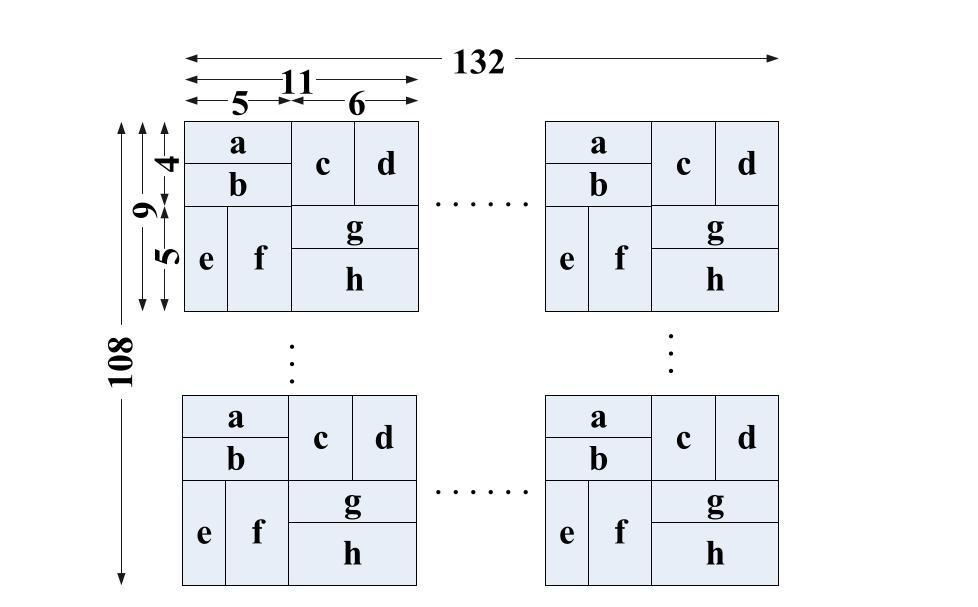
\includegraphics[width=\textwidth]{dados/figuras/divisaosceneframe.jpg}
    \caption{Divisão da imagem para cálculo dos elementos diferenciais. Referência: \citeauthor{mao2015sceneframe}}
\end{figure}

\subsection{Diminuição do espaço de memória utilizado}

O artigo também propõe uma alternativa para diminuir o espaço de memória utilizado para armazenar as assinaturas, visto que o banco de dados dos vídeos pode ser grande. Para isso, é proposta uma técnica chamada qualificação quaternária, na qual os valores são classificados de acordo com um \textit{threshold}.



